\documentclass{article}
\usepackage{listings}
\usepackage{amsmath}
\usepackage{fullpage}
\usepackage{tabularx}
\usepackage{graphicx}
\usepackage{tikz}
\usepackage{cite}
\usepackage{hyperref}
\begin{document}
\lstset{language=python, tabsize=4}
\title{Graph mining: deep learning approaches}
\author{Yuchen Hou}
\maketitle

\begin{abstract}
	I summarize recent deep learning approaches in 2 graph mining tasks: node prediction and link prediction. The key in all these approaches is node embedding(the process of representing every node in the graph as a point in a node space, i.e. embedding nodes in node space), and the coordinates of the point are expected to contain most information about the node related to the prediction task. Equivalently, in this process, every node is represented by a node vector(a 1D numerical array). This process is critical because neural nets can only handle numbers directly, which means everything needs to be converted to numbers before it can be processed by a neural net. Other aspects in these approaches are task specific and I will address them in corresponding sections.
\end{abstract}

\section{Introduction}

\subsection{Entities and relations in different domains}
Deep learning architectures built from neural nets have achieved wide spread success in 3 domains: speech recognition, image recognition, and natural language processing. In order to understand how it can handle prediction tasks in graph mining, first we take an overview on 3 types entities in these 3 domains and 3 types entities in graph mining. \autoref{tab:domains} provides a summary of these entities, their representations in neural nets and inter-entity relation examples.

\begin{table}[h]
	\centering
	\begin{tabularx}{\textwidth}{ |c|c|c|X| }
		\hline domain & entity & representation & relations to other entities \\ 
		\hline image recognition & image & 2D pixel array & NA \\ 
		\hline speech recognition & utterance & 2D spectrogram array & NA \\ 
		\hline natural language processing & word & word vector(1D array) & relations to other words \\ 
		\hline graph mining & movie & node vector(1D array) & produced by producer, directed by director, etc \\ 
		\hline graph mining & user & node vector(1D array) & rate movies, message other users, etc \\ 
		\hline graph mining & article & node vector(1D array) & address topics, cite other articles, etc \\
		\hline
	\end{tabularx}
	\caption{A summary of various types of entities, their representations and inter-entity relations in different domains: images and utterances can be directly represented by 2D numerical arrays, but have no strong relations to other images or utterances; words and various types of nodes in graphs are  hypothetically represented by 1D numerical arrays(which will be verified later), but have strong relations to other words and nodes. Notice that the representations for all the entities are numerical arrays, because neural nets rely on neurons' activations and communications, which are both numerical.}
	\label{tab:domains}
\end{table}

\subsection{Representations of entities in different domains}
In \autoref{tab:domains}, the entities listed in the lower rows have increasing representation complexities. Pixel and spectrogram arrays for images and utterances can be measured by physical instruments from the entities themselves. \autoref{fig:Airy-pattern} shows how an image is represented by a 2D pixel intensity array in image recognition. \autoref{fig:Spectrogram-19thC} shows how an utterance is represented by a 2D spectrogram array in speech recognition. Notice that beside the differences in their axes, these 2 representations have little difference.

\begin{figure}[h]
	\centering
	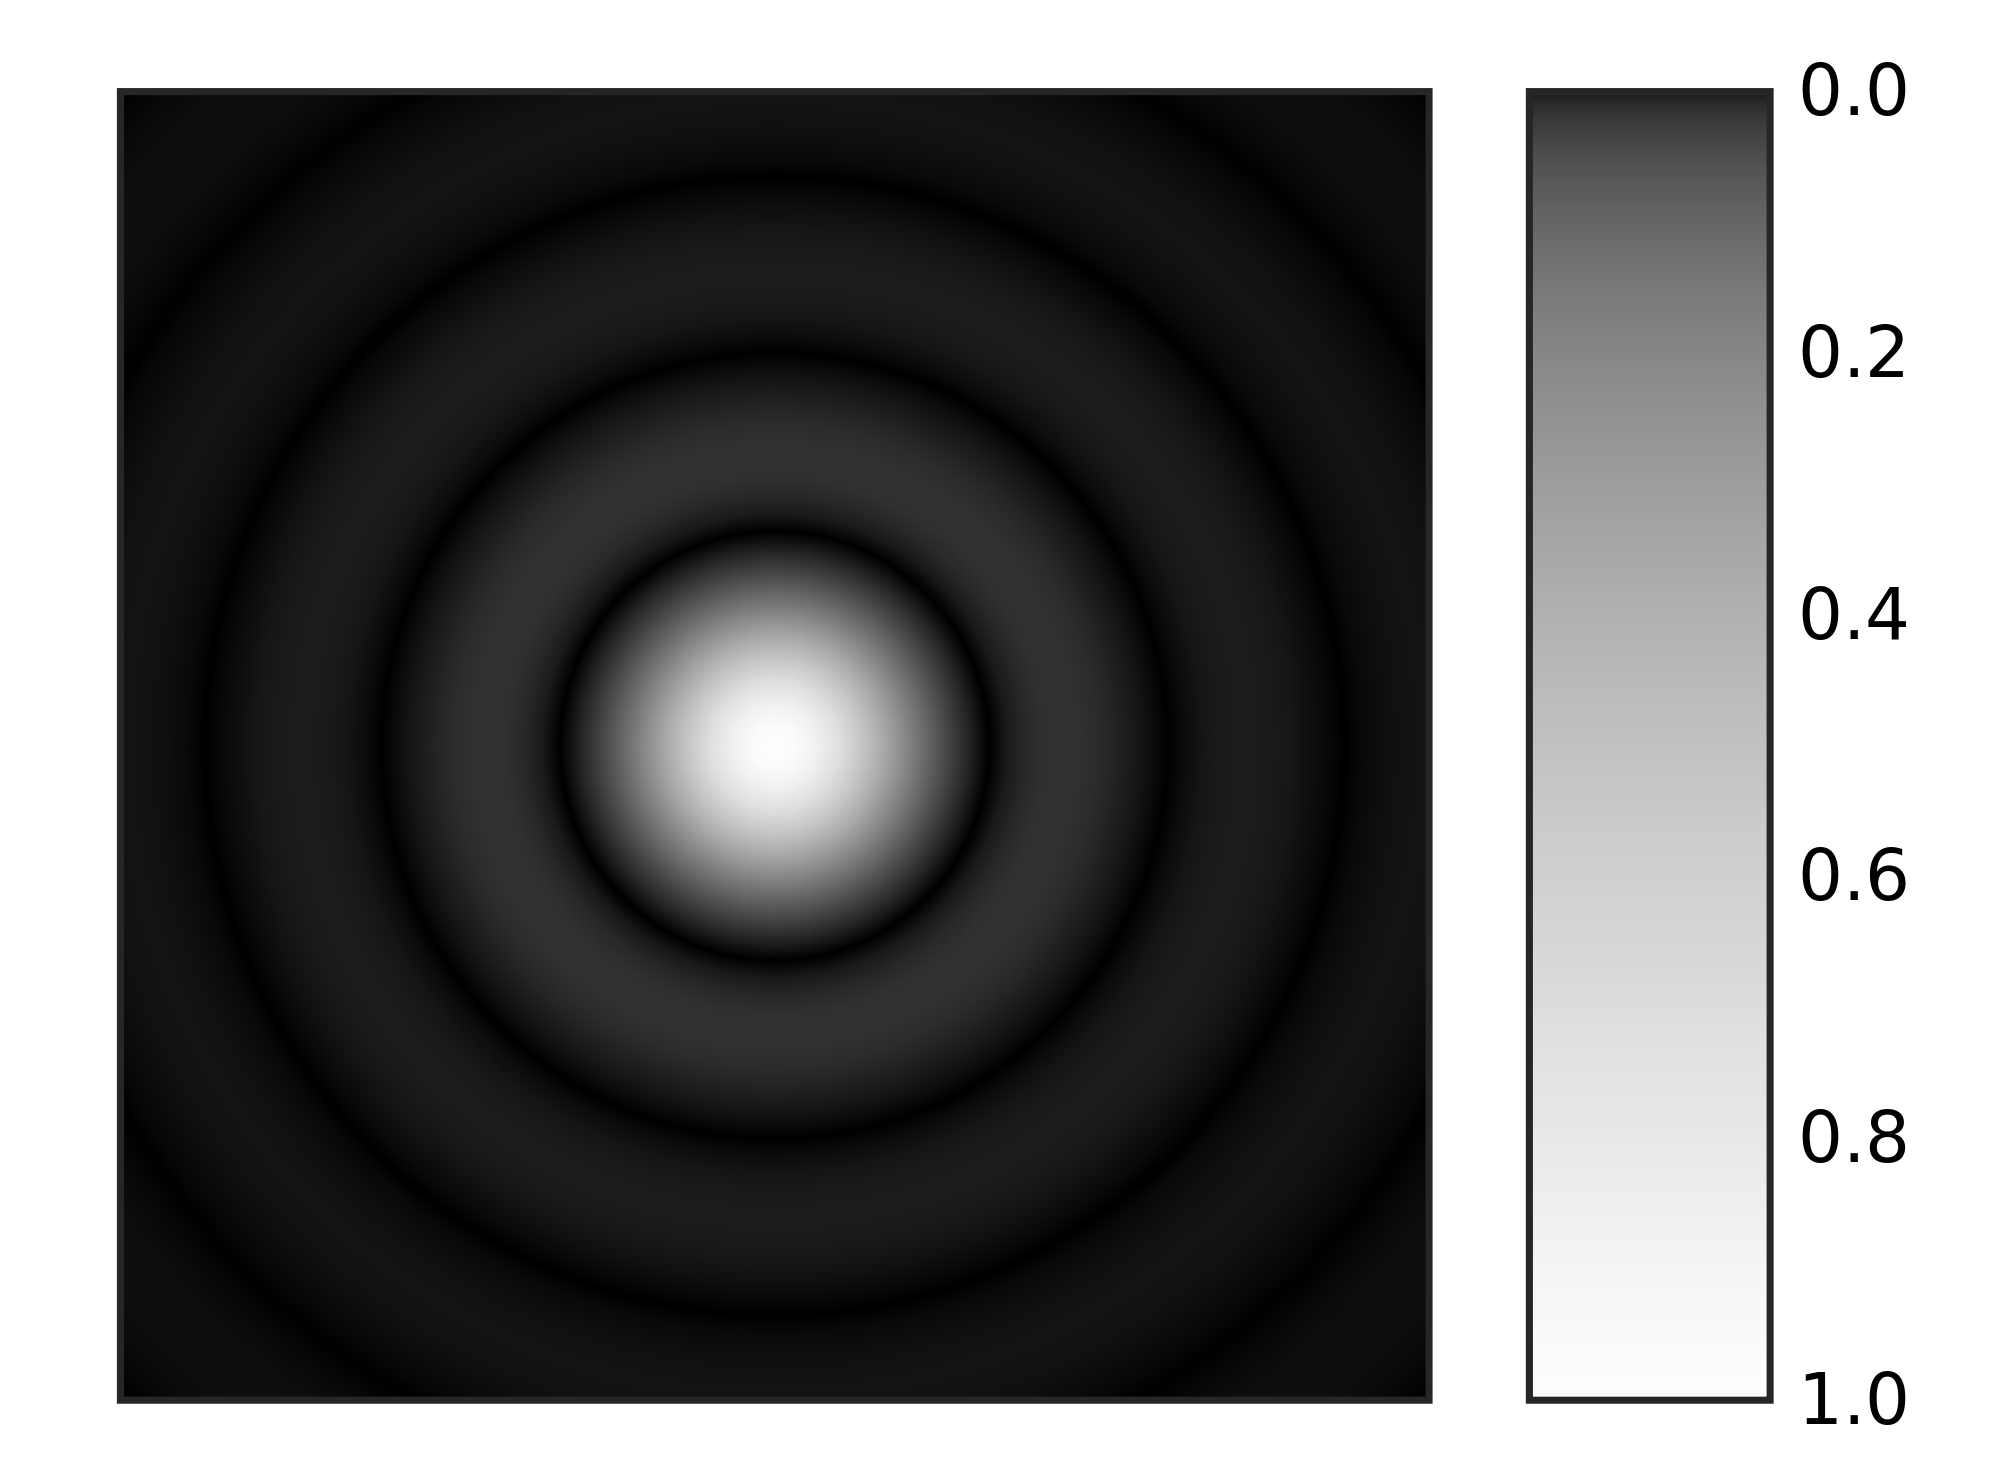
\includegraphics[width=0.5\linewidth]{Airy-pattern}
	\caption{The 2D pixel array of an image of  \href{https://commons.wikimedia.org/wiki/File:Airy-pattern.svg}{the airy pattern} (John Doe / Wikimedia Commons / Public Domain): the horizontal and vertical axes represent the width and the height; the numerical value at a specific (width, height) location is the pixel intensity in range(0, 1).}
	\label{fig:Airy-pattern}
\end{figure}

\begin{figure}[h]
	\centering
	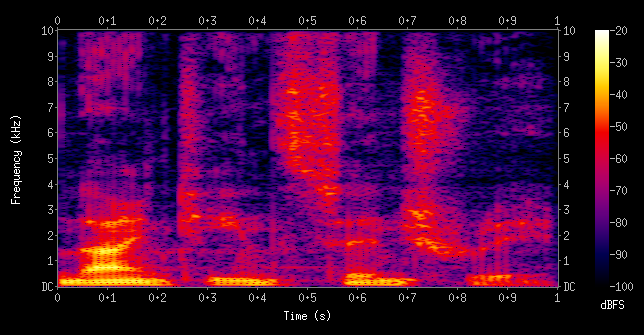
\includegraphics[width=\linewidth]{Spectrogram-19thC}
	\caption{The 2D spectrogram array of \href{https://commons.wikimedia.org/wiki/File:Spectrogram-19thC.png}{a male voice saying [nineteenth century]}(Aquegg / Wikimedia Commons / Public Domain): the horizontal and vertical axes represent the time and frequency; the numerical value at a specific (time, frequency) location is the sound intensity measured in unit dBFS(decibel relative to full scale).}
	\label{fig:Spectrogram-19thC}
\end{figure}

If words and nodes can be represented by numerical arrays like those for images and utterances, neural nets will be able to handle challenging prediction tasks in these 2 domains using these numerical arrays. Now the question is how to achieve this representation. Interestingly, it turns out neural net itself has the capability to do it. In the next few sections I summarize node embedding and a few different deep learning approaches in graph mining:
\begin{itemize}
	\item Section 2: word embedding in natural language processing????(the foundation for node embedding) .
	\item Section 3: node embedding in graph mining and node classification.
\end{itemize}

\section{Word embedding in natural language processing}
In this section, I summarize word embedding(representing every word in a vocabulary with a word vector) introduced in \cite{mikolov2013efficient}, which is used as the foundation of node embedding in \cite{perozzi2014deepwalk}.

\subsection{The goal}

In order to apply neural nets to perform prediction tasks in natural language processing, we want to be able to represent each word in the vocabulary with a word vector. We expect the information about this word (its relations with other words) be stored in this vector, so that a neural net can use it to perform prediction tasks like language modeling. Word vectors are more difficult to get compared to 2D arrays of images and utterances. This is because no instrument can measure words and produce the vector; instead every word vector can only be learned from its relations to other words in the corpus. \autoref{tab:word} shows how each word in a vocabulary is represented by a 1D array which we call word vector.

\begin{table}[h]
	\centering
	\begin{tabularx}{0.5\textwidth}{|c|c|X|} \hline
		rank & word & word vector \\ \hline
		1 & the & [2.3, 564, -9.5 ... 3] \\ \hline
		2 & be & [76, -342.2, 0.3 ... 4.2] \\ \hline
		3 & to & [-345, -834, 0.3 ... 34] \\ \hline
		... & ... & ... \\ \hline
		n & $ word_n $ & $ [x_1, x_2, x_3 ... x_d] $ \\ \hline
	\end{tabularx}
	\caption{1D arrays of words in English sorted by the popularity of the words: there are n words in the entire vocabulary; each word is represented by a 1D array of size d; the numerical values in this table are hypothetical, which will be learned in real applications.}
	\label{tab:word}
\end{table}

\subsection{Application scenario}

Once word embedding is accomplished, neural nets can use the resulting word vectors to perform prediction tasks. The application discussed in the paper is language modeling. The dataset is a corpus in which every word can be any one of the n words in a finite vocabulary. The prediction task is: given a sequence X of t words, predict the next word Y. In other words, both X and Y can be viewed as random variables and we want to find the conditional probability:
\begin{equation}
P(Y = w_t|X = (w_0, w_1, w_2 ... w_{t-1}))
\end{equation}
where w's are words indexed by their ordering in the corpus. In the simplest case, we don't want to find the above possibility for every word; we only want to find the word that has the maximum possibility:
\begin{equation}
	w = argmax_{w_t}P(Y = w_t|X = (w_0, w_1, w_2 ... w_{t-1}))
\end{equation}

\subsection{Observations and the approach}

It's easy to see why word vectors can be learned from relations between words manifested in word co-occurrences within a corpus. In any word sequence, we refer the surrounding words of word w the context of w. For example, the sequence [guard, peace, and, justice, in, the, universe], its word and its context are shown below:
\begin{itemize}
	\item sequence = [guard, peace, and, justice, in, the, universe]
	\item word = [justice]
	\item context = [guard, peace, and, in, the, universe]
\end{itemize}
Every word in the context is related to [justice] in some way and these relations provide information about it. For example, [guard] describes its attribute of existing condition: justice exists if there are those who protect it; otherwise evil will destroy it. As another example, [peace] describes its attribute of virtue: justice is morally good and desirable, like peace. Now it's very clear that words in the context of a word w provides information about different attributes of w. A stronger statement is: every word w can be defined by words in all its contexts within the corpus. In fact, this is also how exactly every dictionary define words - describing a word using other related words. As a follow-up to the previous sequence example, this is the definition of the word [Jedi] provided by Google Dictionary: [a member of the mystical knightly order in the Star Wars films, trained to guard peace and justice in the universe]. Apparently, we can understand this phenomenon in 2 ways:
\begin{enumerate}
	\item words in the contexts of a word describe its relations with other words
	\item words in the contexts of a word describe its attributes
\end{enumerate}
No matter which one is better, we have the observation that related words provide all the information about a word we can possibly get from a corpus. Therefore, it's a good idea to learn the word vector for each word supervised by the words in its contexts.

\subsection{Implementation}

\subsubsection{Skip-gram model}
The paper uses skip-gram neural net model to learn the word vectors. In order to take advantage large corpora, skip-gram model trades off some accuracy for high learning speed by minimizing its neural net complexity to only 3 fully connected layers with formation [n, d, n], where n is the vocabulary size and d is the embedding size. An example model with n=8 and d=4 is shown in \autoref{fig:skipGram}. In fact, skip-gram model is a shallow neural net. The ith unit in the embedding layer has linear activation function:
\begin{equation}
	y_i = f_i(x) = v_i \cdot x
	\label{eq:linear}
\end{equation}
where $ v_i $ and x are the weight vector and the input vector with dimension n. The ith unit in the output layer has softmax activation function:
\begin{equation}
	y_i = f_i(x) = \frac{exp(v_i \cdot x)}{\sum_{i = 1}^{n}exp(v_i \cdot x)}
\end{equation}
where $ v_i $ and x are the weight vector and the input vector with dimension d. Notice that these symbols are not related to those in \autoref{eq:linear}. Also notice that although $ g_i(x) $ is easily implementable, $ f_i(x) $ is not. What I show here is a conceptual illustration - the real implementation has more optimized and complex structure.

\begin{figure}[h]
	\centering
	\newcommand{\layersep}{2.5cm}
	\newcommand{\vocabularySize}{8}
	\newcommand{\embeddingSize}{4}
	\begin{tikzpicture}[shorten >=1pt,->,draw=black!50, node distance=\layersep]
	\tikzstyle{every pin edge}=[<-,shorten <=1pt]
	\tikzstyle{neuron}=[circle,fill=black!25,minimum size=17pt,inner sep=0pt]
	\tikzstyle{input neuron}=[neuron, fill=green!50];
	\tikzstyle{output neuron}=[neuron, fill=red!50];
	\tikzstyle{hidden neuron}=[neuron, fill=blue!50];
	\tikzstyle{annot} = [text width=4em, text centered]
	
	% Draw the input layer
	\foreach \name / \y in {1,...,\vocabularySize}
	% This is the same as writing \foreach \name / \y in {1/1,2/2,3/3,4/4}
	\node[input neuron, pin=left:$ w_\y $] (I-\name) at (0,-\y) {};
	
	% Draw the hidden layer
	\foreach \name / \y in {1,...,\embeddingSize}
	\path[yshift=-2cm]
	node[hidden neuron] (H-\name) at (\layersep,-\y cm) {};
	
	% Draw the output layer
	\foreach \name / \y in {1,...,\vocabularySize}
	\node[output neuron, pin={[pin edge={->}]right:$ w_\y $}] (O-\name) at (2*\layersep,-\y) {};
	
	% Connect the input layer with the hidden layer
	\foreach \source in {1,...,\vocabularySize}
	\foreach \dest in {1,...,\embeddingSize}
	\path (I-\source) edge (H-\dest);
	
	% Connect the hidden layer with the output layer
	\foreach \source in {1,...,\embeddingSize}
	\foreach \dest in {1,...,\vocabularySize}
	\path (H-\source) edge (O-\dest);
	
	% Annotate the layers
	\node[annot,above of=H-2] {embedding layer};
	\node[annot,above of=I-2] {input layer};
	\node[annot,above of=O-2] {output layer};
	\end{tikzpicture}
	
	\caption{The skip-gram model with vocabulary size 8 and embedding size 4: the model consists of only 3 layers - an input layer with one-hot activation, an embedding layer of linear units, and an output layer of softmax units. For example, given sequence = [$ w_3, w_2, w_8, w_1, w_4 $], we have input word = [$ w_8 $] and output context = [$ w_1, w_2, w_3, w_4 $]. The input layer has activation = (0, 0, 0...0, 1), where $ w_8 $ is 1 and others are 0; the output layer has activation = (1, 1, 1, 1, 0 ... 0), where $ w_1, w_2, w_3, w_4 $ are 1 and others are 0. The weights in the embedding layer are the word vectors shown in \autoref{tab:word}. For example, the word vector for $ w_8 $ are the weights in the embedding layer units connected to $ w_8 $ These weights are randomly initialized and learned by the neural net during training. The embedding layer's activation is equal to the word vector of the current word due to one-hot activation in the input layer.}
	\label{fig:skipGram}
\end{figure}

\subsubsection{Learning algorithm}
The paper uses the de facto standard learning algorithm for neural net: stochastic gradient descent with back propagation\cite{lecun2012efficient}.

\section{Node embedding in graph mining}

In this section, I summarize node embedding(representing every node in a graph with a node vector) introduced in \cite{perozzi2014deepwalk}.

\subsection{The goal}

The goal of node embedding is identical to word embedding: to represent nodes with node vectors so that a neural net can use it. Similar to word vectors shown in \autoref{tab:word}, node vectors are shown in \autoref{tab:node}.

\begin{table}[h]
	\centering
	\begin{tabularx}{0.5\textwidth}{|c|c|X|} \hline
		ID & node & node vector \\ \hline
		1 & A & [2.3, 564, -9.5 ... 3] \\ \hline
		2 & B & [76, -342.2, 0.3 ... 4.2] \\ \hline
		3 & C & [-345, -834, 0.3 ... 34] \\ \hline
		... & ... & ... \\ \hline
		n & $ word_n $ & $ [x_1, x_2, x_3 ... x_d] $ \\ \hline
	\end{tabularx}
	\caption{1D arrays of user nodes in a graph sorted by the node ID: there are n nodes in the entire graph; each node is represented by a 1D array of size d; the numerical values in this table are hypothetical, which are learned in real applications.}
	\label{tab:node}
\end{table}

\subsection{Application scenario}

Once word embedding is accomplished, neural nets can use the resulting word vectors to perform prediction tasks. The application mentioned in the paper is node classification. The dataset is a graph in which links do not have attributes but every node can have any number of the n labels in a finite label set. More formally, every node has one attribute - a list of n boolean variables where each variable indicates whether the node has a particular label. For example,
\begin{lstlisting}
node[4].attribute = [ture, false, false... true]
\end{lstlisting}
means $ node_4 $ has $ label_0 $, has no $ label_1 $, has no $ label_2 $... and has $ label_n $. The attribute values are known for a portion of nodes, which serve as training data. The prediction task is: given a node X, predict its attribute value Y(determine which labels it has).

\subsection{Observations and the approach}

By comparing the data in natural language processing and that in graph mining, we can observe their similarities, shown in \autoref{tab:word_vs_node}. Most importantly, a sentence is very similar to a walk.

\begin{table}[h]
	\centering
	\begin{tabularx}{\textwidth}{ |X|X|X| } \hline
		aspect  & natural language processing & graph mining \\ \hline
		information source & text & graph \\ \hline
		basic entities & words & nodes \\ \hline
		entity collection & vocabulary & node set \\ \hline
		relations between entities & collocations (implicit) & links (explicit) \\ \hline
		entity sequences & sentences(word sequences) & walks(node sequences) \\ \hline
	\end{tabularx}
	\caption{A comparison of natural language processing and graph mining from several aspects: the similarity of these 2 domains across all these aspects makes it possible to reduce node embedding to word embedding.}
	\label{tab:word_vs_node}
\end{table}

As neural nets can represent every word in a vocabulary based on the relations between words in word sequences in natural languages (sentences), in the same way it should be able to represent every node in the node set based on the links between nodes in node sequences in the graph (walks). Based on these observations, the node vectors can be learned supervised by the nodes in the random walk.

\subsection{Implementations}
The paper implement node embedding the same way as word embedding discussed in previous section. The node sequences are random walks sampled from the graph. After the the neural net learned the word vectors, the output layer replaces the softmax units with logistic regression units to perform label prediction task. Its neural net has 3 fully connected layers with formation [n, d, l], where n is the node set size, d is the embedding size and l is the label set size. An example model with n=8, d=4 and l=2 is shown in \autoref{fig:label}. This model is a shallow neural net. The ith unit in the output layer has logistic regression activation function:
\begin{equation}
y = f(x) = \frac{1}{1 + exp(-v_i \cdot x)}
\end{equation}
where $ v_i $ and x are the weight vector and the input vector with dimension d. Notice that during this stage, only the activation layer update its weight during the learning, while the embedding layer does not. Otherwise, the node vectors learned from previous node embedding stage will be destroyed.

\begin{figure}[h]
	\centering
	\newcommand{\layersep}{2.5cm}
	\newcommand{\vocabularySize}{8}
	\newcommand{\embeddingSize}{4}
	\newcommand{\labelSetSize}{2}
	\begin{tikzpicture}[shorten >=1pt,->,draw=black!50, node distance=\layersep]
	\tikzstyle{every pin edge}=[<-,shorten <=1pt]
	\tikzstyle{neuron}=[circle,fill=black!25,minimum size=17pt,inner sep=0pt]
	\tikzstyle{input neuron}=[neuron, fill=green!50];
	\tikzstyle{output neuron}=[neuron, fill=red!50];
	\tikzstyle{hidden neuron}=[neuron, fill=blue!50];
	\tikzstyle{annot} = [text width=4em, text centered]
	
	% Draw the input layer
	\foreach \name / \y in {1,...,\vocabularySize}
	% This is the same as writing \foreach \name / \y in {1/1,2/2,3/3,4/4}
	\node[input neuron, pin=left:$ node_\y $] (I-\name) at (0,-\y) {};
	
	% Draw the hidden layer
	\foreach \name / \y in {1,...,\embeddingSize}
	\path[yshift=-2cm]
	node[hidden neuron] (H-\name) at (\layersep,-\y cm) {};
	
	% Draw the output layer
	\foreach \name / \y in {1,...,\labelSetSize}
	\node[output neuron, pin={[pin edge={->}]right:$ label_\y $}] (O-\name) at (2*\layersep,-\y) {};
	
	% Connect the input layer with the hidden layer
	\foreach \source in {1,...,\vocabularySize}
	\foreach \dest in {1,...,\embeddingSize}
	\path (I-\source) edge (H-\dest);
	
	% Connect the hidden layer with the output layer
	\foreach \source in {1,...,\embeddingSize}
	\foreach \dest in {1,...,\labelSetSize}
	\path (H-\source) edge (O-\dest);
	
	% Annotate the layers
	\node[annot,above of=H-2] {embedding layer};
	\node[annot,above of=I-2] {input layer};
	\node[annot,above of=O-2] {output layer};
	\end{tikzpicture}
	
	\caption{The label prediction model with node set size 8, embedding size 4 and label set size 2: the model consists of only 3 layers - an input layer with one-hot activation, an embedding layer of linear units, and an output layer of logistic regression units. For example, given input node = [$ node_8 $] and output label = [$ label_1 $]. The input layer has activation = (0, 0, 0...0, 1), where $ w_8 $ is 1 and others are 0; the output layer has activation = (1, 0), where $ label_1 $ is 1 and $ label_2 $ is 0. The weights in the embedding layer are the node vectors shown in \autoref{tab:node}. In this stage, the units in embedding layer already have all node vectors learned and will not update the weights; only the unites in output layer will update their weights.}
	\label{fig:label}
\end{figure}

\subsection{Strengths of this approach}

\subsubsection{Representing nodes as node vectors}
In terms of information flow, we can understand this approach of graph mining as a node-centric approach, as information about nodes is extracted from links connecting these nodes and then stored in nodes. In a social network scenario where we want to understand a user, this means who a user contacts and what a user does tells us what kind of person he is. This fits many real world graphs well: usually a graph has complex entities with unobservable attributes which we represent as nodes; it also has simple interactions/relations between these entities with observable attributes which we represent as links, as shown in \autoref{tab:nodes_vs_links}.

\begin{table}[h]
	\centering
	\begin{tabularx}{0.5\textwidth}{ |c|c|X| } \hline
		aspect  & node & link \\ \hline
		complexity & high & low \\ \hline
		attribute observability & low & high \\ \hline
	\end{tabularx}
	\caption{A comparison of node and link with respect to their complexity and attribute observability: links tend to have low complexity and high attribute observability while nodes are the opposite. In a social network example, it's easy to observe simple user activities like sending messages other users, leaving comments on posts and give ratings to music, but it's hard to observe complex user attributes like personality, style or taste in music.}
	\label{tab:nodes_vs_links}
\end{table}

\subsubsection{Online learning}
The training samples in this approach are walks in the graph. Every walk is randomly generated, then fed to the neural. During this training step, the neural net extract the information provided by this walk and use it to update the node vector. After this training step,  the random walk can be discarded. Therefore, the learning is incremental and only requires samples of different walks in the graph, not the construction or storage of the complete graph. In streaming graph settings, it is sufficient to keep a finite number of latest links streamed in inside the memory, just enough to sample walks of reasonable lengths.

\subsection{Weaknesses of this approach}

\subsubsection{Node sequence generation}

The node sequence generation with random walks on the graph is likely a weakness, although these sequences shares 3 similarities with word sequences used by very successful skip-gram model. These similarities are listed and explained below:
\begin{enumerate}
	\item Sentences and walks are both very natural sequences. Skip-gram model uses sentences because they are the only available data in corpora, not because this provides special benefits to the model. Furthermore, most of the words in the context of a word are usually related to it so using sentences doesn't not have much negative effect to skip-gram. However, the situation is not the same for walks in graph. First, sampling nodes from long walks in the graph is not the only option; a more computational efficient one is to sample nodes from the neighborhood of the node. Also, a deep walk is likely to sample remote nodes, which are not strongly related to the root node.
	\item Words and nodes in the sequences have informative ordering. Although the ordering is significant in both cases, they are 2 different types of orderings. In a sentence, words are ordered to make the sentence correct and meaningful, not to make more similar words closer to each other. For example, in sentence [The quick brown fox jumps over the lazy dog.], [quick] and [brown] are very close but they are in fact very unrelated words; [fox] and [dog] are very far but they are strongly related words. Fortunately, his undesirable phenomena doesn't have negative effect on skip-gram model, because skip-gram model is not capable to pick up word ordering information anyway. This is not the case in a node sequence, where nodes with closer distances in the graph usually have closer distances in the sequence. This ordering is very critical and contains information we want skip-gram model to capture, but its indifference to ordering makes this impossible.
	\item The frequency distribution of words and nodes follow power law. This one is bad for both cases, which should be avoided instead of taken advantage of. For example, skip-gram model can get useful information from co-occurrences of 'capital' and 'Beijing', but not so much from co-occurrences of 'the' and 'capital'. Here 'the' is a prominent example word with very high frequency but provides little information about anything. Frequent words like 'the' reduce both the speed and accuracy of learning word embedding, and are intentionally discard with sub-sampling technique in natural language processing \cite{mikolov2013distributed}.
\end{enumerate}

\subsubsection{Information loss during node embedding}
Another weakness is that node attribute is not used in the node embedding process. If every node with known attribute value can have that information embedded in its node vector, this information can propagate to nodes with unknown attribute values in the random walk and embeds in their node vectors. In this way, every node vector can contain more valuable information.

\subsubsection{Unable to use rich attributes in graph}
The fundamental weakness in this node embedding approach is that it is unable to use information provided by node and link attributes in many real world graphs. One feature of this approach is that it can produce good node vectors when the available information about the graph is limited to the topology. This feature becomes a weakness when rich node attributes and link attributes provide much more information than topology of the graph does. Graphs can have many measurable attributes and also many types of relations to other entities. For example, a user has attributes like age, weight, salary, DNA sequence, and has relations with other entities like rating songs, writing articles, messaging other users. Every one of these attributes and relations provides useful information about what kind of person the user is and potentially useful in a prediction task like whether this user would be interested in a specific song or article. \autoref{fig:weakness} illustrates this weakness using a simple example in a movie rating prediction scenario.

\begin{figure}[h]
	\centering
	\newcommand{\layersep}{8}
	\newcommand{\vocabularySize}{3}
	\newcommand{\embeddingSize}{5}
	\begin{tikzpicture}[shorten >=1pt,->,draw=black!50, node distance=\layersep]
	\tikzstyle{every pin edge}=[<-,shorten <=1pt]
	\tikzstyle{neuron}=[circle, draw, minimum size=20]
	\tikzstyle{input neuron}=[neuron];
	\tikzstyle{output neuron}=[neuron];
	\tikzstyle{hidden neuron}=[neuron];
	\tikzstyle{annot} = [text width=4em, text centered]
	
	% Draw the input layer
	\foreach \name / \y in {1,...,\vocabularySize}
	\node[input neuron] (I-\name) at (0,-2*\y) {$ user_\name $};
	
	% Draw the hidden layer
	\foreach \name / \y in {1,...,\embeddingSize}
	\path[yshift=2cm]
	node[hidden neuron] (H-\name) at (\layersep,-2*\y) {$ movie_\name $};
	
	% Connect the input layer with the hidden layer
	\foreach \source in {1,...,\vocabularySize}
	\foreach \dest in {1,...,\embeddingSize}
	\path (I-\source) edge (H-\dest);
	\end{tikzpicture}
	
	\caption{The weakness of solely relying on topology and ignoring graph attributes: in a graph where users rate movies, users and movies are represented as nodes and ratings are represented as links. In this paper, the node embedding approach is not able to use the link attribute - the rating values. Therefore, if 3 users have rated the same 5 movies, they will have same node vector due to the topology, even if they give very different ratings to each movie. This makes the node vectors useless to perform any prediction task.}
	\label{fig:weakness}
\end{figure}


\section{Node prediction:others}

\section{Link prediction}

\subsection{Graphs with rich node attributes and link attributes}
In some prediction tasks, graphs need to incorporate rich attributes in nodes and links to take advantage of large amount of available information. This becomes significant in scenarios where a service provider allows a wide range of activities from the users and record these activities. The popular Amazon e-commerce service is a good example, which records these activities as available information:
\begin{enumerate}
	\item buyers can buy, rate, write reviews, post questions and answers for products, and rate, write reviews for sellers, 
	\item manufactures produce, write descriptions for products
	\item sellers sell, write advertisements for products
\end{enumerate}
Beside these activities, buyers, manufactures and sellers have very limited information about themselves in their profile, while products have richer information like price, category, specs. Having all this comprehensive information in hand, it is of great interest to the service provider to.

\bibliographystyle{acm}
\bibliography{references}

\end{document}